\documentclass[1pt, a4paper]{article}

\input{structure.tex}


\begin{document}
\maketitlepage
\tableofcontents
\newpage
\noindent
\section{Functional requirement of the program}
\noindent
All the functions which are used for the computing or the displaying of the results are called in the main file. At first there are the functions wich create the initial values in respect of the parameters set in the settings file, then this values are stocked in data (.dat) files in a directory named "parameters". With these data files, we don't have to repeat the calculations every time we want to test something. Then you have the functions that compute the results (the phase of the oscillators, the complex mean average, and the Shannon entropy), wich are stocked in data files in the same directory. And finally there are the functions that display the graphs by using the module \py{matplotlib.pyplot}. In this section we will describe the functions that create the datas files and their datas. Firstly the initial datas are created throught the \py{class Data} wich is in the data file. Finally the computing of the other values is in the \py{class KuramotoModel} wich is in the kuramoto file.
\subsection{The initialisation of the datas}
The initial datas are created by the function: \py{data.init_data(state)}. You can choose if you want to create new initial datas by changing the boolean value of the \py{newData=False} variable in the settings file.
\begin{table}[htbp]
    \begin{center}
        \begin{tabular}{p{0.3\linewidth} p{0.3\linewidth} p{0.3\linewidth}} \toprule
            \multicolumn{3}{c}{\py{data.init_data(state="random")}}\\
            \midrule
            \hfil Description & \hfil Input & \hfil Output\\
            \cmidrule(r){1-1} \cmidrule{2-2} \cmidrule(l){3-3}
           
            This function is using to create initial values, stocked in data files in the directory parameters, according to the value of the argument \py{state} set by default to \py{state="random"}. You can create data for random, chimera, inverse, or josephson states. &
            The argument \py{state} is a \py{string}. By default it takes the value \py{"random"} but you can give it these values:\begin{itemize}[leftmargin=15pt]
            \setlength{\itemsep}{0pt}
            \item \py{"random"}
            \item \py{"chimera"}
            \item \py{"inverse"}
            \item \py{"josephson"}
            \end{itemize}
            & This function will retrieve you six data file in the parameters directory, computing in according to the \py{state} argument.
            The data files are: \begin{itemize}[leftmargin=15pt, itemsep=0pt]
            \item \py{"omega.dat"}
            \item \py{"theta0.dat"}
            \item \py{"K.dat"}
            \item \py{"eta.dat"}
            \item \py{"alpha.dat"}
            \item \py{"tau.dat"}
            \end{itemize}\\
            \bottomrule
        \end{tabular}
    \end{center}
    \caption{function data.init\_data()}
    \label{tab:init_data}
\end{table}\\
Each \py{state} create six variables, wich are defined as follows:
\begin{itemize}
        \item $\omega$ is a list of real of size N. It contains the natural oscillations of each oscillators.
        \item $\theta_0$ is a list of real of size N. It contains the intial phase of each oscillators. So at the $\theta^i(t=t_0)$.
        \item $K$ is a matrix of real of size NxN. It contains the coupling coefficients between each oscillators depending on the nearest neighbour. The nearest neighbour of an oscillator are defined by M in the settings file. It is set as $30\%$ of the totality of the oscillators, you can change it. 
        \item $\alpha$ is a matrix of real of size NxN. It is the dephasing matrix of the coupling.
        \item $\tau$ is a matrix of real of size NxN. It is the delay matrix.
        \item $\eta$ is a matrix of real of size NxT. It is the representations of external noises for each oscillators at each time $t\in ]0, T[$.
\end{itemize}
They are different for each state, you can see their definitions in the tables \ref{tab:states1} and \ref{tab:states2}. The function \py{uniform()} is from the module \py{random}, and provide random real numbers with uniform distribution, in the range given. The function \py{randint()} do the same things but for integers.
\begin{table}[htbp]
    \begin{center}
        \begin{tabular}{p{0.40\linewidth} p{0.40\linewidth}} \toprule
            \hfil \py{"random"} & \hfil \py{"chimera"}\\
            \cmidrule(r){1-1} \cmidrule(l){2-2}
            This \py{state} represent the case with random values defined by:
            \begin{itemize}[leftmargin=15pt, itemsep=0pt]
                \item $\omega^i=uniform(0, 3)$
                \item $\theta_0^i=uniform(0, \dfrac{2}{\pi})$
                \item $K^i_j=uniform(0, 1e10)$
                \item $\eta^i_j=uniform(0, 0.5)$
                \item $\alpha^i_j=uniform(0, \dfrac{2}{\pi})$
                \item $\tau^i_j=randint(0, N//2)$
            \end{itemize}
            &This \py{state} represent the case of a quantum chimera state\cite{chimera} defined by:
            \begin{itemize}[leftmargin=15pt, itemsep=0pt]
               \item $\omega^i=0.2 + i * 0.4 * sin(\dfrac{i^2 * \pi}{(2 * N^2)})$
               \item $\theta_0^i=uniform(0, \dfrac{2}{\pi})$
               \item $K^i_j=uniform(0, 1e10)$
               \item $\eta^i_j=uniform(0, 0.5)$
               \item $\alpha^i_j=1.46$
               \item $\tau^i_j=randint(0, N//2)$
            \end{itemize}\\
            \bottomrule
        \end{tabular}
    \end{center}
    \caption{\py{states}}
    \label{tab:states1}
\end{table}
\begin{table}[htbp]
    \begin{center}
        \begin{tabular}{p{0.40\linewidth} p{0.40\linewidth}} \toprule
            \hfil \py{"inverse"} & \hfil \py{"josephson"}\\
            \cmidrule(r){1-1} \cmidrule(l){2-2}
            This \py{state} represent the case with the coupling matrix defined by the inverse of the distance between two oscillators, and the delay matrix is proportionnal to this distance. 
            \begin{itemize}[leftmargin=15pt, itemsep=0pt]
                \item $\omega^i=uniform(0, 3)$
                \item $\theta_0^i=uniform(0, \dfrac{2}{\pi})$
                \item \begin{equation*}
                K^i_j=\left\{\begin{array}{ll}
                    \dfrac{1}{\abs{i-j}}\;if\;\abs{i-j} \neq 0\\
                    1e20\;otherwise
                \end{array}\right.
            \end{equation*}
                \item $\eta^i_j=uniform(0, 0.5)$
                \item $\alpha^i_j=1.46$
                \item $\tau^i_j=\abs{i-j}$
            \end{itemize}
            &This \py{state} represent the case of the array of Josephson, the datas were drawn from this article \cite{josephson}. Their datas are defined by:
            \begin{itemize}[leftmargin=15pt, itemsep=0pt]
               \item $\omega^i=0.2 + 0.4i\times sin(\dfrac{i^2\pi}{(2N^2)})$
               \item $\theta_0^i=uniform(0, \dfrac{2}{\pi})$
               \item $K^i_j=\dfrac{Nr\omega^{i^2}2\e/(\hbar rI_b)-\omega^i}{\sqrt{(L\omega^{i^2} - 1/C)^2 + \omega^{i^2}(R+rN)^2 }}$
               \item $\eta^i_j=uniform(0, 0.5)$
               \item $cos(\alpha^i_j)=\dfrac{L\omega^{i^2} - 1/C}{\sqrt{(L\omega^{i^2} - 1/C)^2 + \omega^{i^2}(R+rN)^2 }}$
               \item $\tau^i_j=randint(0, N//2)$
            \end{itemize}\\
            \bottomrule
        \end{tabular}
    \end{center}
    \caption{\py{states}}
    \label{tab:states2}
\end{table}
\newpage
\noindent
For each \py{state} choosen you have to define in the settings file the parameters \py{Nr} and \py{Nc}, to define the geometry of the system. \py{Nr} define the number of rows and \py{Nc} the number of columms, so \py{N=Nr*Nc} is the number of oscillators that you have. For example if you choose \py{N=12} in the geometry \py{Nr=3, Nc=4}, you will have this configuration:\\
\begin{figure}[htbp]
    \centering
    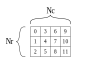
\includegraphics[scale=0.8]{figure/os_table.pdf}
    \caption{Configuration of the oscillators for \py{Nr=3, Nc=4}}
    \label{fig:os_table}
\end{figure}\\
\noindent
The labels in the Figure are the labels of the oscillators. If you put a non-positive number you will have some issues, the program will not work. So be careful to respect the physics of the system.
\subsection{The computing functions}
\noindent
There are three computing functions that are imported from the \py{class KuramotoModel}, by the object \py{kuramoto}. You can choose if you want to compute new datas by changing the boolean value of the \py{newComputing=False} variable in the settings file.
\begin{table}[htbp]
    \begin{center}
        \begin{tabular}{p{0.3\linewidth} p{0.3\linewidth} p{0.3\linewidth}} \toprule
            \multicolumn{3}{c}{\py{kuramoto.integrate(f, theta0, tf=100, integrator="RK4")}}\\
            \midrule
            \hfil Description & \hfil Input & \hfil Output\\
            \cmidrule(r){1-1} \cmidrule{2-2} \cmidrule(l){3-3}
           
            This function compute integrates the function \py{f}, with the initial vector \py{theta0} during a time \py{tf}, set by default to \py{tf=100} with 1000 values, using the integrator, set by default to \py{integrator="RK4"}&
            \begin{itemize}[leftmargin=15pt, itemsep=0pt, topsep=0pt ]
            \item \py{f} is the function to be integrated, such that $f:\real^n  \rightarrow  \real^n$
            \item \py{theta0} is the initial vector, such that $\theta_0 \in \real^n$. So it has to be a list of real of size N
            \item \py{tf} is the duration of the integration. Set to 100 by default. It is an integer
            \item \py{integrator} is the integrator that you want to choose. It can take only this string values: \py{"Euler"}, \py{"RK2"}, \py{"RK4"}. Among the three integrators, RK4 is the one losing the least energy the longer the integration lasts, therefore it is the default value.
            \end{itemize}
            & \\
            \bottomrule
        \end{tabular}
    \end{center}
    \caption{function kuramoto.integrate()}
    \label{tab:integrate}
\end{table}\\

\newpage
\bibliographystyle{plain}
\bibliography{biblio}

\end{document}
